\documentclass{beamer}
\usetheme{CambridgeUS}
\usepackage[utf8]{inputenc}

\usepackage{xcolor}
\usepackage{minted}

\usepackage{caption}
\captionsetup[figure]{labelformat=empty}% redefines the caption setup of the figures environment in the beamer class.

\usemintedstyle{friendly}

\title[iCLIP data analysis with iCount]
{Analysis of iCLIP data with the iCount python module}
\subtitle{
    A short tutorial
}
 
\author[Tomaž Curk]{
    Tomaž Curk\\
    \small{tomaz.curk@fri.uni-lj.si}
}
\institute[UL FRI]{
    University of Ljubljana\\
    Faculty of Computer and Information Science
}

\titlegraphic{
\includegraphics[height=2cm]{images/ul-fri.png}}

\date[The Crick Institute, 14. 7. 2017]
{The Crick Institute, July 2017}

\newif\ifplacelogo % create a new conditional
\placelogofalse % set it to false

\logo{\ifplacelogo
\includegraphics[height=0.8cm]{images/ul-fri.png}\fi}


\begin{document}

\frame{\titlepage}


\section{Background}
\begin{frame}
\frametitle{History and acknowledgements for iCount}
From its start in late 2008, a great number of people contributed to the development of
iCount.

In mid-2016, Jure Zmrzlikar from Genialis helped to improve the code, which is now available on
github.

\begin{itemize}
\item Tomaž Curk
\item Gregor Rot
\item Črtomir Gorup
\item Julian Konig
\item Yoichiro Sugimoto
\item Nejc Haberman
\item Goran Bobojević
\item Jure Zmrzlikar
\item Christian Hauer
\item Matthias Hentze
\item Blaž Zupan
\item Jernej Ule
\end{itemize}
\end{frame}

\begin{frame}
\frametitle{Pipeline}

\begin{figure}
\begin{center}
    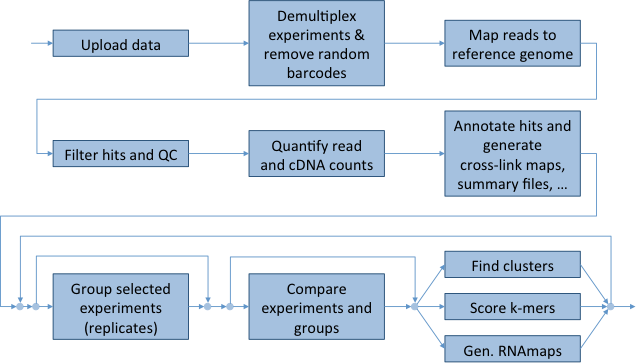
\includegraphics[width=0.85\linewidth]{images/pipeline.png}
    \caption{Main steps in the cross-link mapping and annotation pipeline.}
\end{center}
\end{figure}

\end{frame}


\begin{frame}
\frametitle{Finding cross-linked sites}

\begin{figure}
\begin{center}
    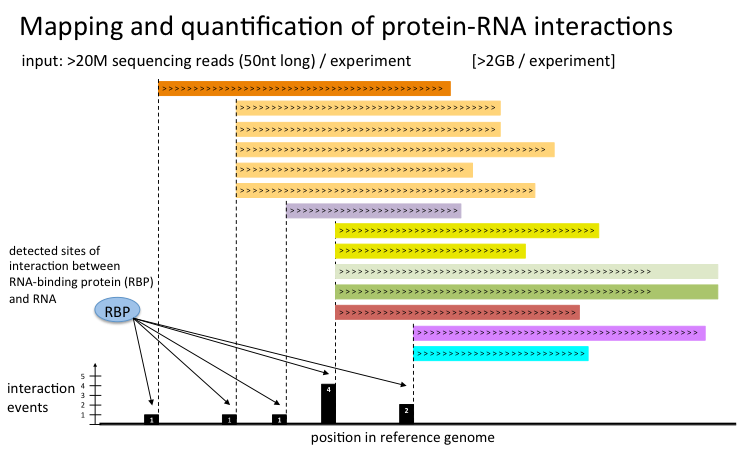
\includegraphics[width=0.85\linewidth]{images/mapping.png}
    \caption{The most crucial step is site indetification and quantification.}
\end{center}
\end{figure}

\end{frame}


\begin{frame}
\frametitle{The old web interface}

\begin{figure}
\begin{center}
    \centering
    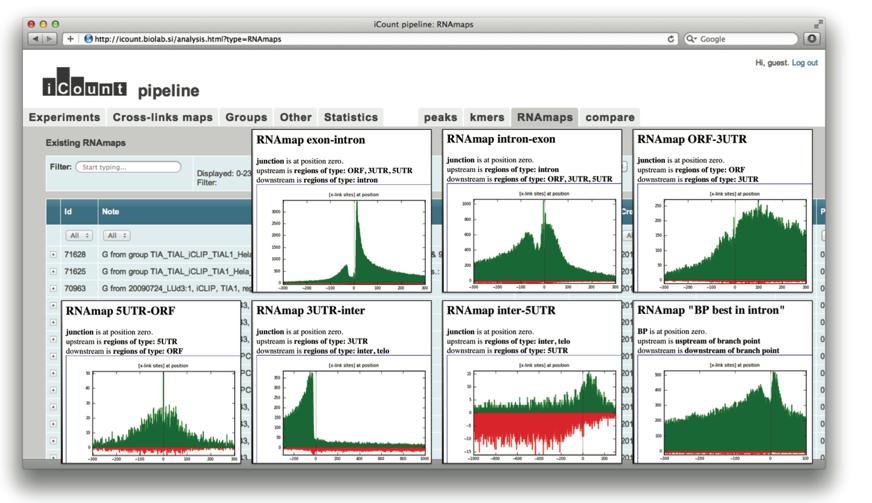
\includegraphics[width=0.85\linewidth]{images/old_webinterface.png}
    \caption{This interface is still in use.\\
    It will be replaced soon by an implementation by Genialis.}
\end{center}
\end{figure}

\end{frame}


\begin{frame}
\frametitle{The old iCount - impact}

\begin{itemize}
\item 100+ users
\item 40+ institutions: UCL, MRC LMB, EMBL, mpi-cbg.de, …
\item 2M+ EUR cost of sequencing alone
\item 80+ proteins (8\% of known human RBPs)
\item 5000+ experiments (iCLIP, CLIP, pA-Seq, mRNA-seq,…)
\item 800+ user-defined groupings of experiments
\item 10 species
\item 33000 analyses

\item (Co)authors of over 25 publications using results from iCount.
\end{itemize}

\end{frame}


\section{Today}
\begin{frame}
\frametitle{iCount is available on github!}

\begin{figure}
\begin{center}
    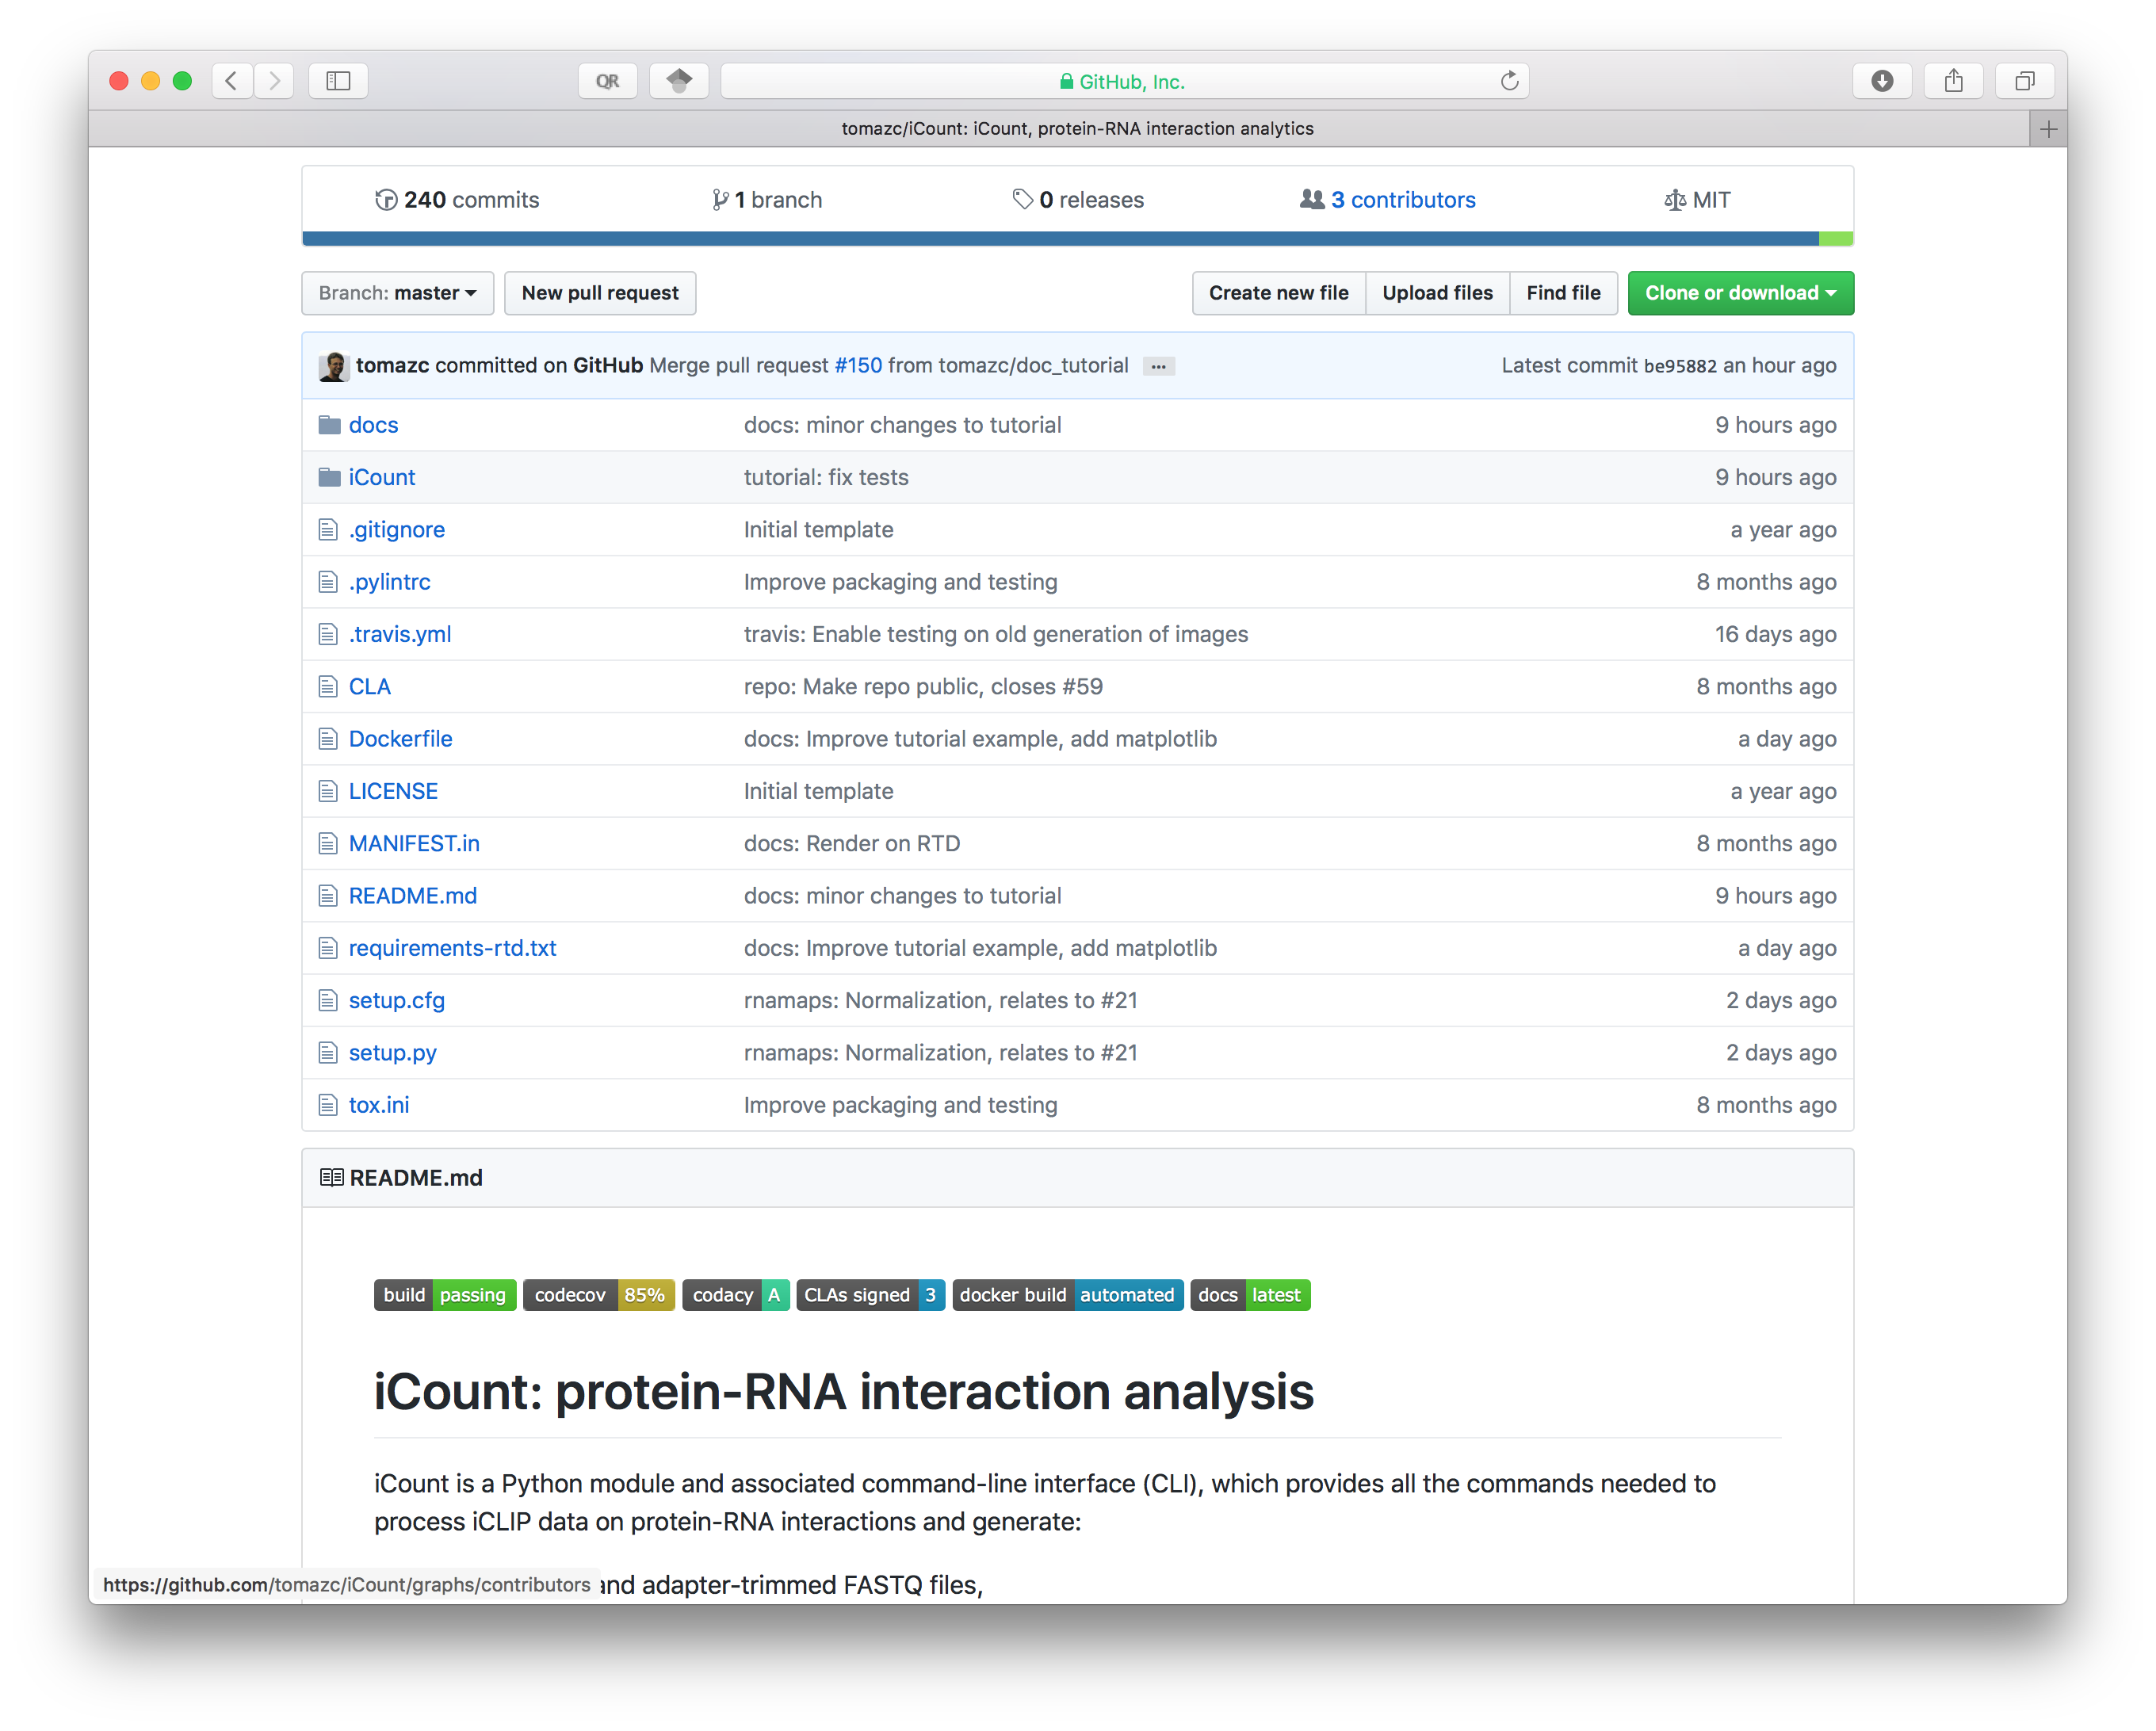
\includegraphics[width=0.6\linewidth]{images/github.png}
    \caption{http://github.com/tomazc/iCount\\
    Comments and PR are welcome!}
\end{center}
\end{figure}

\end{frame}


\section{Tutorial}
\begin{frame}
\frametitle{Tutorial}

\begin{figure}
\begin{center}
    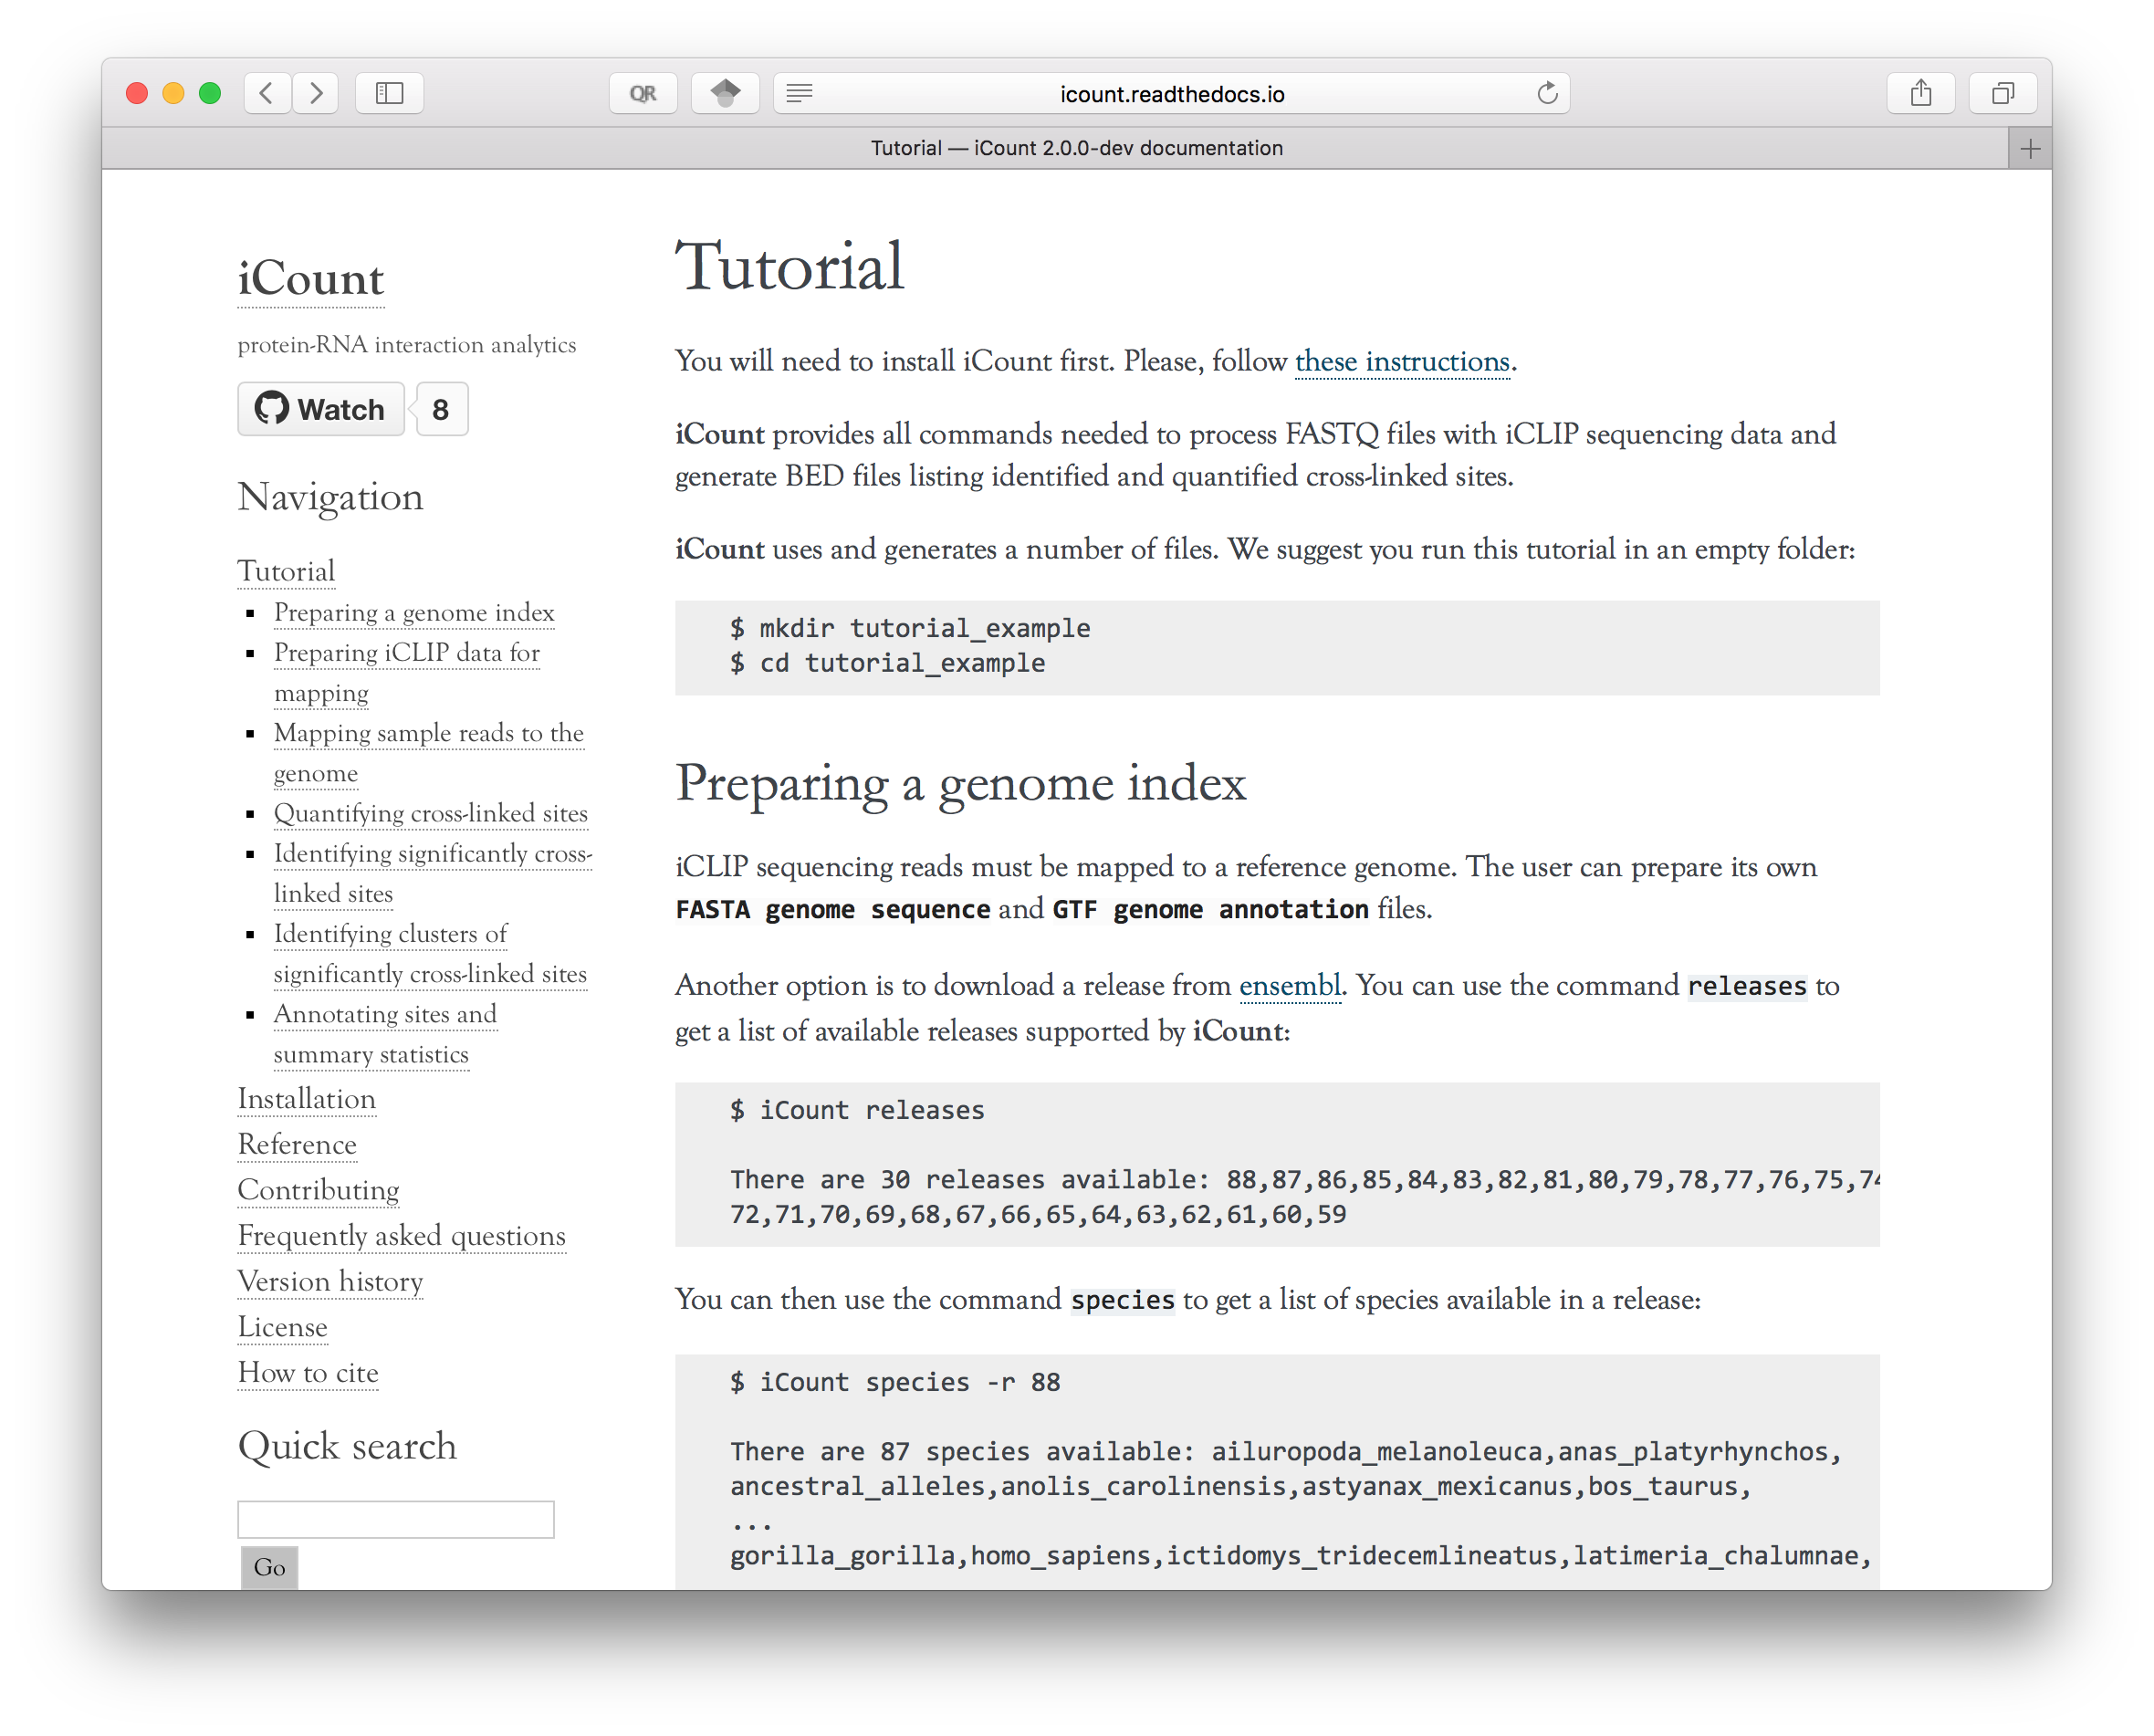
\includegraphics[width=0.65\linewidth]{images/tutorial.png}
    \caption{http://icount.readthedocs.io/en/latest/tutorial.html}
\end{center}
\end{figure}

\end{frame}


\section{Conclusion}

\placelogotrue

\begin{frame}
\frametitle{Use and contribute to iCount}
\centering

In case of problems, post an issue on github or contact: tomaz.curk@fri.uni-lj.si

Welcome to contribute to http://github.com/tomazc/iCount

\end{frame}

\end{document}